% Auteur : Romain TESTUD
\begin{frame}{Wormhole - Mise en contexte}
    \centering
    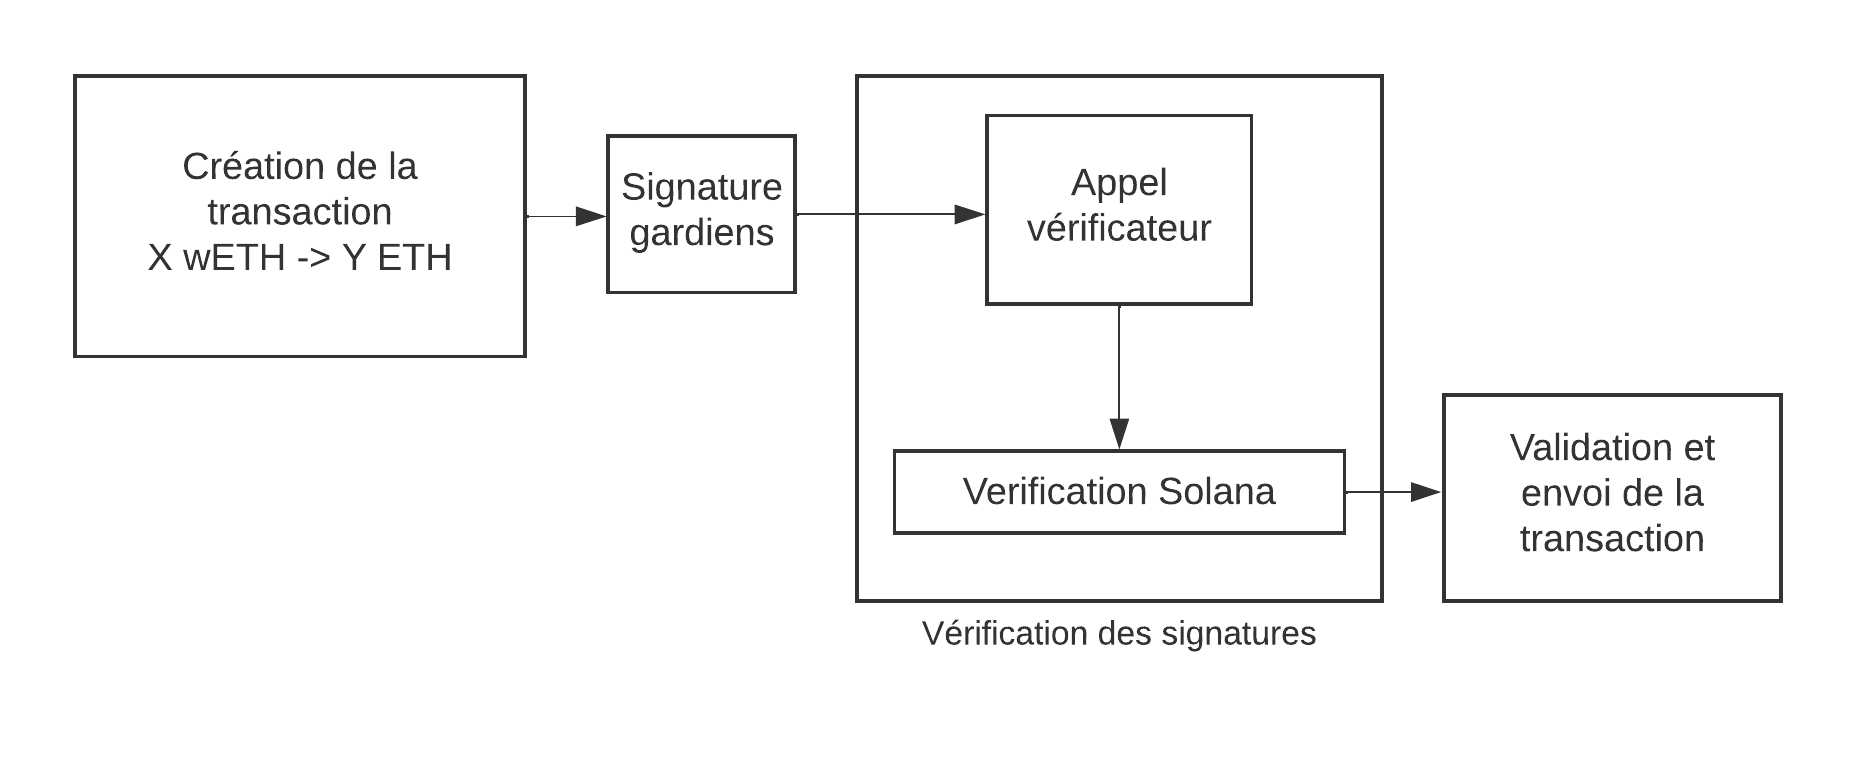
\includegraphics[scale = 0.69]{centralisation/img/wormhole/worm_fonc.png}
\end{frame}

\begin{frame}{Wormhole - Mise en contexte}
    \begin{itemize}
        \item Transaction standard.
    \end{itemize}
        \centering
        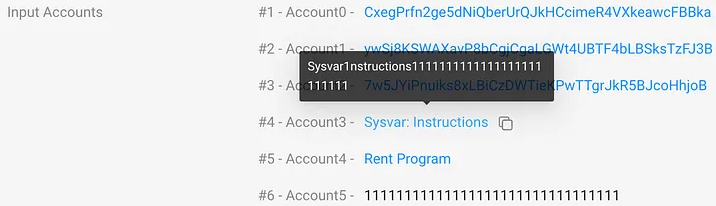
\includegraphics[scale = 0.45]{centralisation/img/wormhole/sysvar_trans_normal.png}
\end{frame}
%\begin{frame}{Le protocole Wormhole}
%    \begin{block}{Mise en contexte}
%        \begin{itemize}
%            \item Solution d'échanges inter-blockchains.
%            \item utilisation de bridges.
%        \end{itemize}
%    \end{block}
%    \begin{block}{Les étapes d'un transfert}
%        \begin{itemize}
%            \item Formulation de la transaction.
%            \item Récupération et vérification des signatures des gardiens.
%            \item Envoi de la transaction.
%        \end{itemize}
%    \end{block}
%    \begin{figure}
%        \centering
%        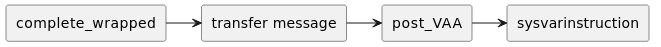
\includegraphics[scale = 0.3]{centralisation/img/fonctions.png}
%        \caption{Fonctions appelées lors d'un transfert}
%    \end{figure}
%\end{frame}

\begin{frame}{Wormhole - L'attaque}
    \begin{block}{Attaque sur le bridge entre Solana et Ethereum}
        \begin{itemize}
            \item Le 2 Février 2022.
            \item 120 000 ETH (300M \$) de perte.
            \item Correction de bug publiée mais pas encore en production.
        \end{itemize}
    \end{block}
    \begin{block}{L'attaquant a contourné\dots}
        \begin{itemize}
            \item la signature des gardiens.
            \item la vérification des signatures. 
        \end{itemize}
    \end{block}
\end{frame}

\begin{frame}{Wormhole - L'attaque}
    \centering
    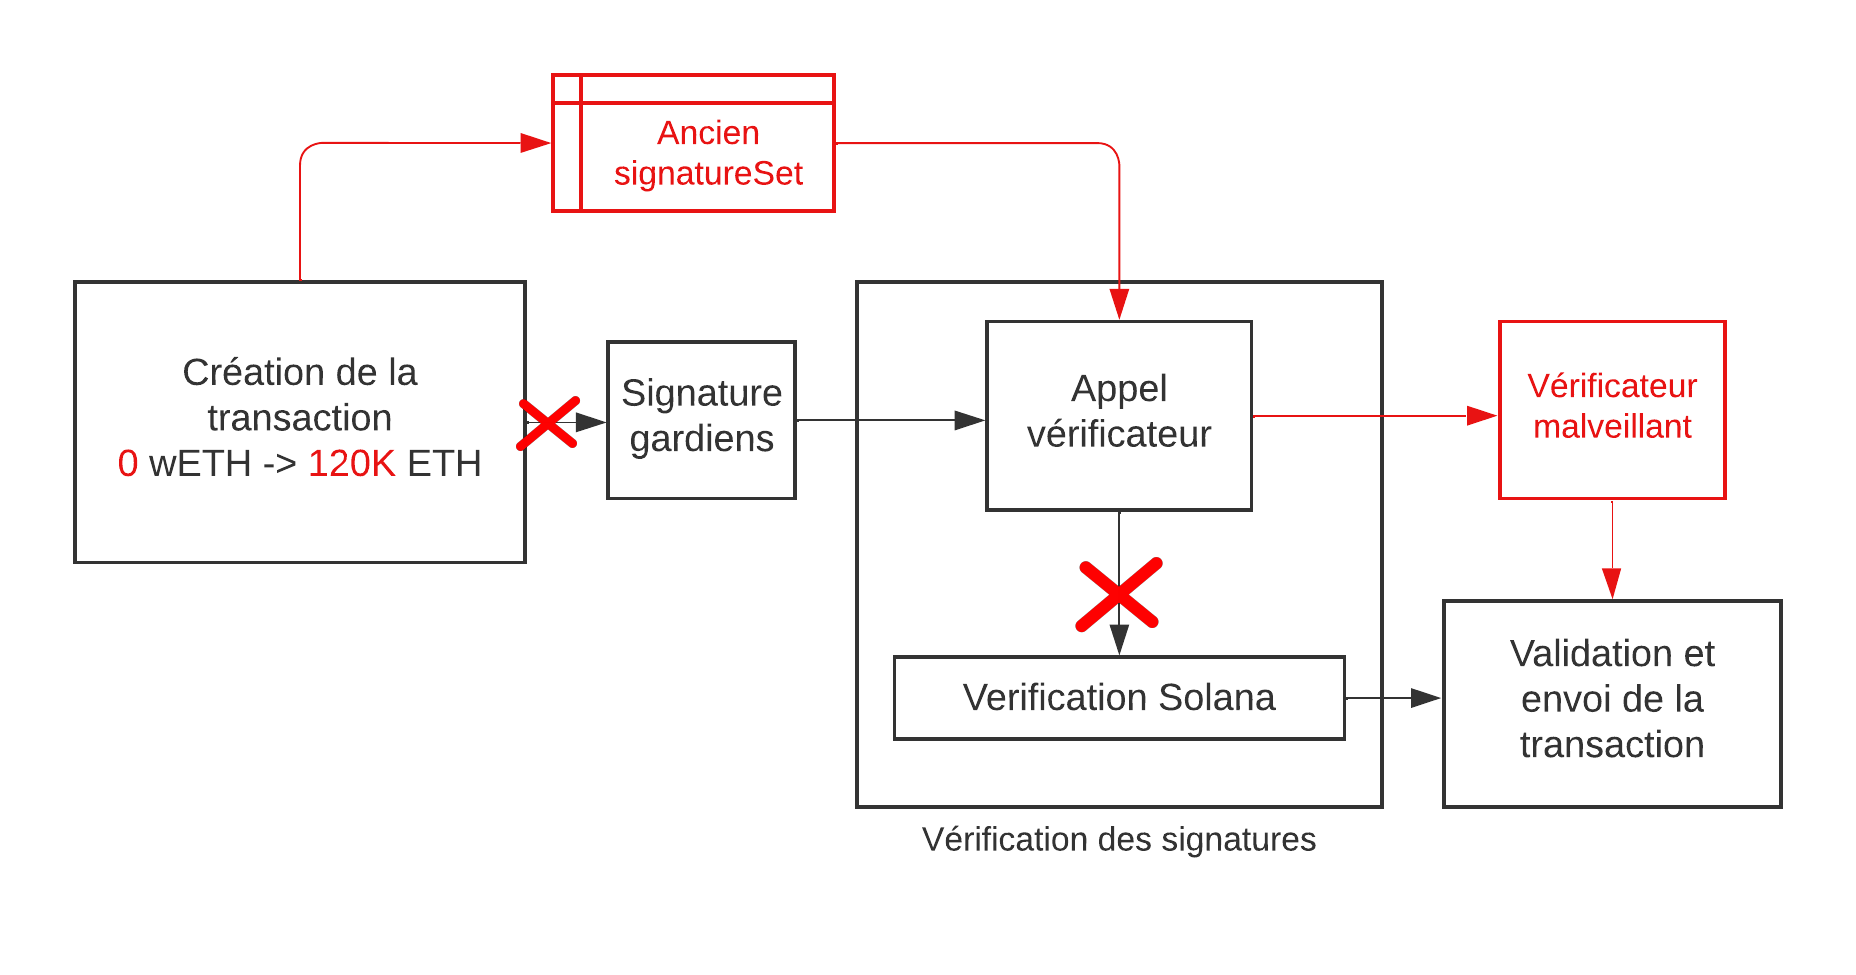
\includegraphics[scale=0.69]{centralisation/img/wormhole/worm_hack.png}
\end{frame}

%\begin{frame}{L'attaque}
%    \begin{block}{Passer la signature des gardiens?}
%        Utilisation de signatures d'une transaction antérieure.
%    \end{block}
%    \begin{block}{Passer la vérification ?}
%        \begin{itemize}
%            \item Exploitation d'une erreur d'implémentation dans \textit{verify\_signature}
%            \item Appel à un programme externe.
%        \end{itemize}
%        \begin{figure}
%            \centering
%            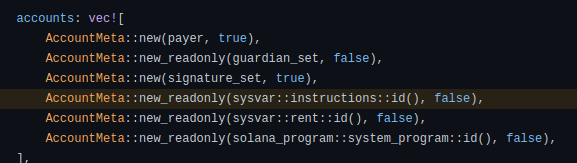
\includegraphics[scale = 0.3]{centralisation/img/sysvar_atk.png}
%            \caption{Appel à la fonction de vérification}
%        \end{figure}
%    \end{block}
%\end{frame}



\begin{frame}{Wormhole - L'attaque}
    \begin{itemize}
        \item Transaction de l'attaquant.
    \end{itemize}
        \centering
        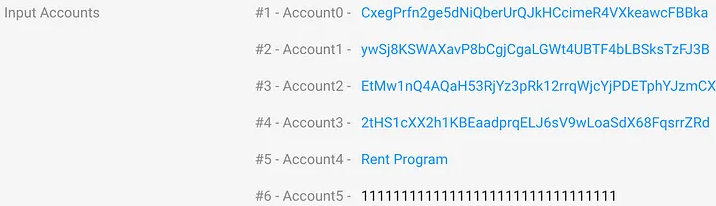
\includegraphics[scale = 0.45]{centralisation/img/wormhole/sysvar_transaction_hack.png}
\end{frame}

\begin{frame}{Wormhole - L'attaque}
    \begin{block}{Transaction validée et envoyée}
        \begin{itemize}
            \item 120 000 ETH transmis.
            \item 0 wETH déposés.
        \end{itemize}
    \end{block}
    \begin{block}{Correctif}
        Vérification des appels externes.\\
        \centering
        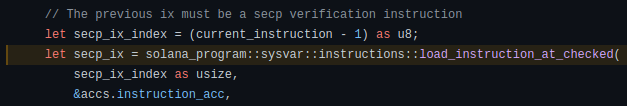
\includegraphics[scale = 0.5]{centralisation/img/wormhole/worm_fixed.png}
    \end{block}
\end{frame}

%\begin{frame}{Correctif}
%    \begin{itemize}
%        \item Vérification de l'appel par \textit{sysvar\_instruction}
%    \end{itemize}
%    \begin{figure}
%        \centering
%        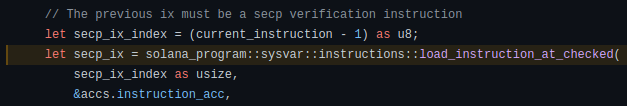
\includegraphics[scale = 0.3]{centralisation/img/wormhole/worm_fixed.png}
%        \caption{Appel à la fonction de vérification}
%    \end{figure}
%\end{frame}